% Paper draft for FPGA 2013
\documentclass{acm_proc_article-sp}
\usepackage{graphicx}
\usepackage{multirow}
\usepackage[caption=true,font=footnotesize]{subfig}
\usepackage{dblfloatfix}
\usepackage{algorithmic}
\usepackage{algorithm}
\usepackage{xspace}
\usepackage{url}
%\renewcommand{\topfraction}{0.5}
%\renewcommand{\dbltopfraction}{0.5}

\renewcommand\floatpagefraction{.9}
\renewcommand\topfraction{.9}
\renewcommand\bottomfraction{.9}
\renewcommand\dbltopfraction{.9}
\renewcommand\textfraction{.1}   
\setcounter{totalnumber}{50}
\setcounter{topnumber}{50}
\setcounter{bottomnumber}{50}

\newcommand{\eqnref}[1]{(\ref{#1})}
\newcommand{\figref}[1]{Figure~\ref{#1}}
\newcommand{\algref}[1]{Algorithm~\ref{#1}}
\newcommand{\secref}[1]{Section~\ref{#1}}
\newcommand{\tabref}[1]{Table~\ref{#1}}

\newcommand{\autoesl}{AutoESL\xspace}

\usepackage{etoolbox}
\makeatletter
\patchcmd{\maketitle}{\@copyrightspace}{}{}{}
\makeatother
\graphicspath{{./figures/}}

\begin{document}

\title{Automatic Nested Loop Acceleration On A Highly Predictable Soft Coarse-Grained Reconfigurable Array Overlay}

\numberofauthors{1}
 \author{
% % 1st. author
 \alignauthor
 xxx\\
 \affaddr{The University of Hong Kong}\\
 \email{xxx@hku.hk}
% % 2nd. author
% \alignauthor
% name2\\
%        \affaddr{Electrical and Electronic Engineering}\\
%        \affaddr{The University of Hong Kong}\\
%        \email{email2}
% % 3rd. author
% \alignauthor
% name3\\
%        \affaddr{Electrical and Electronic Engineering}\\
%        \affaddr{The University of Hong Kong}\\
%        \email{email3}
 }

%\author{}
\maketitle

\begin{abstract}
We present an automatic hardware/software co-design framework for accelerating a nested loop on a 
hybrid CPU+FPGA system. It partially unrolls the inner loop, maps the unrolled part to a soft 
coarse-grained reconfigurable array (SCGRA) overlay based FPGA accelerator built on top of the 
off-the-shelf FPGAs and generates corresponding drivers to utilize the FPGA accelerator to complete
the whole loop. It will delicately leverage the communication cost and computation benefits on 
FPGA and the users can acquire an optimal co-design by simply providing the high-level 
user constraints such as energy and hardware resource budgets instead of 
manually improving the hardware and software design repeatedly. In addition, as the SCGRA based FPGA 
accelerator has highly predictable hardware overhead, power consumption and performance, the design 
space exploration (DSE) becomes fast and easy to converge. According to the experiments, it takes 5 
minutes to 30 minutes to complete the DSE for each application of the benchmark.

\end{abstract}
 
% A category with the (minimum) three required fields
%\category{H.4}{Information Systems Applications}{Miscellaneous}
% A category including the fourth, optional field follows...
%\category{D.2.3}{Hardware Engineering}{Metrics}[complexity measures, performance measures]
%\terms{Theory}
%\keywords{High Level Synthesis, Soft Coarse Grain Reconfigurable Array, Design Productivity, High Frequency FPGA Design}

%\section{Introduction}
Offloading compute intensive nested loops to FPGA accelerators has 
been demonstrated as an effective way of performance 
acceleration across various application domains\cite{Chung2010}. 
However, the design productivity of developing such accelerators 
remains relatively low and it has become a major obstacle that 
hinders the wide adoption of FPGAs as compute engines. Although the use of 
high level synthesis (HLS) tools which allow the application designers to 
focus on high level functionality instead of low-level implementation details alleviates 
this shortcoming \cite{cong2011high}, the lengthy low-level FPGA implementation process 
greatly limits the number of compile-debug-edit cycles per day and dramatically 
affects the overall design productivity. 

To approach the above design productivity problem, 
researchers have recently turned to the use of virtual FPGA overlay 
architectures \cite{Grant2011Malibu,ZUMA2012,mesh-FUs,
ferreira2011fpga, kissler2006dynamically,scgra}. When combined properly to 
high level compilation tools, the overlay architecture based design methods 
are able to produce high-performance accelerators at near software 
compilation speed, but at the cost of hardware overhead, power and even performance.
By customizing the architectures of these \emph{virtual} 
overlays for a target user design, in theory, it is 
possible to significantly improve the performance-energy of the 
resulting accelerator. In practice, however, navigating through a 
labyrinth of architectural and compilation parameters to fine-tune 
an accelerator's performance-energy is a slow and non-trivial process. 
To require a user to manually explore such vast design space is going 
to counteract the productivity benefit of the utilizing overlay 
in the first place.

To obtain both high design productivity and advantages of 
application-specific customization, we have developed a 
soft CGRA (SCGRA) overlay based nested loop acceleration design 
framework. This framework targets a hybrid CPU-FPGA computing system where 
nested loop compute kernels expressed in high-level languages are compiled and 
executed on the SCGRA overlay built on top of FPGAs while the rest of the 
user application remains running on the host CPU. Given high-level design 
goals and design constraints, the framework automatically explores the 
design space and customizes architectural parameters specifically to the 
user application. In addition, the framework also exploits loop unrolling 
and hardware-software communication strategies in combination 
with buffer sizing and partition as performance enhancing techniques.
Once the design goals and constraints are fulfilled, the 
corresponding hardware accelerator and communication interface 
are generated and both the hardware accelerator and software 
are compiled to the hybrid CPU-FPGA system.  

As demonstrated in previous work, both the compilation from nested 
loops to the SCGRA overlay \cite{scgra} and the SCGRA overlay 
implementation \cite{ROB2014} are fast. Meanwhile, the SCGRA 
overlay is highly pipelined and has quite regular tiling structure, 
which makes the hardware overhead, power consumption and even implementation frequency 
highly predictable. Therefore, a multitude of design metrics such as performance 
and energy consumption can be accurately estimated using analytical models when the 
overlay scheduling result is available. And the nested loop specific acceleration problem can be 
reduced to a sub design space exploration centering an NP-complete SCGRA scheduling and 
a following customization with all the potential configurations well estimated. 
While the overlay scheduling depends on much less design parameters, the overall 
customization can be dramatically simplified. Accordingly, the overall design 
framework achieves both rapid compilation and fast application specific 
customization and ensures high design productivity and high performance of the resulting
accelerators at the same time.  

We performed a series of experiments to evaluate the efficiency 
and quality of the proposed design framework using a real-world 
benchmark. Compared to an exhaustive search, the proposed 
customization achieves similar results while reducing its 
runtime by 2 orders of magnitude on average. When compared to 
HLS implementations with moderate manual optimizations that can 
reasonably be expected from a novice user,  
the customized accelerators produced using the proposed framework 
has demonstrated competitive performance as well. 

With that, we consider the main contribution of this work is in the following areas:
\begin{itemize}[nosep]
\item We have developed a rapid customization framework that 
    performs automatic design parameter tuning for SCGRA overlay based 
    nested loop acceleration on a hybrid CPU-FPGA computing system. 
    The result is comparable to an exhaustive design space search while 
    it runs at a fraction of time.
\item We have developed a parametric regular SCGRA overlay template. It can be used 
    to generate FPGA accelerators with predictable implementation 
    frequency, hardware overhead and power consumption, which is essential to 
    both the rapid compilation and customization.
\item We have developed a hierarchy on-chip buffer. It allows flexible 
    buffer partition and makes good use of the efficient lock-step computation 
    of the SCGRA overlay.
\end{itemize}

In \secref{sec:relatedwork}, related work is briefly introduced. 
The overall automatic nested loop acceleration framework is illustrated 
in \secref{sec:acc-framework}. Then SCGRA overlay based FPGA accelerator 
is illustrated in \secref{sec:scgra} and the application-specific customization 
method is further detailed in \secref{sec:customization-method}. 
Experimental results are presented in \secref{sec:result} and limitations are 
discussed in \secref{sec:limitations}. Finally, the paper is 
concluded in \secref{sec:conclusion}.



%\section{Related Work}
To improve the productivity of FPGA designers, researchers have approached the problem both by increasing the abstraction level and by reducing the compilation time.

In the first case, decades of research in FPGA high-level synthesis have already demonstrated their indispensible role in promoting FPGA design productivity \cite{cong2011high}. Numerous design languages and environments \cite{cardoso2010compiling} have been developed to allow designers to focus on high-level functionality instead of low-level implementation details. 

While high-level abstraction may help a designers express the desired functionality, the low-level compilation time spent on synthesis, map, and place-and-route for FPGAs remains a major hindrances to designs' productivity. Researchers have approached the problem from many angles, such as through the use of pre-compiled hard macros \cite{lavin2011} in the tool flow, the use of a partial reconfiguration, modular design flow \cite{Frangieh2010}, and the use of coarse-grained reconfigurable fabrics upgrading the configurability from bit-level to word-level \cite{coole2010intermediate} \cite{ferreira2011fpga}. 

%Particularly, the authors in \cite{coole2010intermediate} proposed to implement an intermedia fabrics (IF) as an virtual device on top of commerical-off-the-shelf (COTS) FPGA devices. The IF has computational units connected through the connection boxes and switch boxes and it is more like a traditional FPGA with word-level configurability. It hides much of the complexity of fine-grained COTS FPGA device and enables great speedup of the placement and routing as well as portability over different FPGA devices. This method follows traditional FPGA design flow, but the idea building an intermedia virtual fabrics over COTS device to reduce the complexity of FPGA synthesis and mapping is meanlingful. The authors in \cite{ferreira2011fpga} developed a heterogeneous CGRA as IF to further reduce the compilation time and improve the performance at the same time. 

Finally, the use of parameterizable VLIW processor array \cite{kissler2006dynamically} and even the many-core processors \cite{Lebedev2010} as a template to FPGA design has also been proposed demonstrating improve productivity with moderate performance degradation.

Building on top of many of the above ideas, we have opted to utilize a fully synchronous soft coarse-grained reconfigurable array as an intermediate step to compiling high-level compute intensive application. Productivity is improved both from the vastly reduced compilation time, as well as from the high-level abstraction provided by the generic LLVM compiler framework we utilized as front-end.

%\input{methodology}
%\section{SCGRA overlay based FPGA acceleration} \label{sec:scgra}
In this work, parametric and scalable SCGRA overlay architectures, 
on-chip buffer structures and loop execution strategies 
have been developed for the nested loop acceleration framework. These 
design choices provide unique opportunity for application specific customization 
and help to achieve better performance-energy trade-off of the resulting accelerators.

\subsection{SCGRA Overlay Based FPGA Accelerator}
\figref{fig:scgra-acc} shows the design of a typical SCGRA overlay 
based FPGA accelerator. In the accelerator, on-chip
memory i.e. IBuf and OBuf are used to buffer the communication 
data between the host CPU and the accelerator. A controller is also 
presented in hardware to control the operations of the accelerator as well as
memory transfers. The SCGRA, which is the kernel computation fabric,
consists of an array of processing elements (PEs) and it achieves the computation 
task through the distributed control words stored in each PE. 

PE is the key design element of the SCGRA overlay. It is simple yet 
highly pipelined which is beneficial to the hardware implementation. At the 
heart of PE is an ALU, which is supported by a multi-port data memory and 
an instruction memory. Three of the data memory's read ports are connected 
to the ALU as inputs, while the remaining ports are sent to the output 
multipliers for connection to neighboring PEs and the optional store paths 
external to the SCGRA overlay. At the same time, this data memory takes input 
from the ALU output, data arriving from neighboring PEs as well as from the 
optional IBuf loading path. The action of the PE is controlled by the AccCtrl unit 
that reads from the instruction memory. Finally a global signal from the AccCtrl 
block controls the start/stop of all PEs in the array.

ALU carries out the computations of the given applications. It can be easily customized 
to support operations of a specified application or a group of applications. The supported
operations are fully pipelined in the ALU and may execute concurrently while they must 
complete in a deterministic number of cycles. Since ALU has only a single output port, 
the scheduler will ensure that there is never conflict at the output.
\begin{figure}[tb]
\center{\includegraphics[width=0.99\linewidth]{scgra-accelerator}}
\caption{SCGRA overlay based FPGA accelerator}
\label{fig:scgra-acc}
\end{figure}

\subsection{Loop execution on the accelerator}
\figref{fig:group-dfg} illustrates how the loop is executed 
on the FPGA accelerator. First of all, data flow graph (DFG) is extracted 
from the loop and then it is scheduled on to the SCGRA overlay based FPGA accelerator. 
Depending on how much the loop is unrolled and transformed to DFG, the DFG may be 
executed repeatedly until the end of the original loop. In addition, data transfers for 
multiple executions of the same DFG are batched into groups as shown in \figref{fig:group-dfg}. 
On the one hand, this technique is used to reduce the number of batching, which further 
helps to amortize the initial communication cost. On the other hand, it also 
results in larger on-chip memory overhead. The proposed customization framework 
can be used to make the right design choices to achieve an optimal design. 

\begin{figure}[tb]
\center{\includegraphics[width=0.95\linewidth]{group-dfg}}
\caption{Loop, group and DFG. The loop will be divided into 
groups. Each group will be partially unrolled and the unrolled part will be 
translated to DFG. IO transmission between FPGA and host CPU is performed 
in the granularity of a group.}
\label{fig:group-dfg}
\end{figure}

\subsection{On-chip buffer structure}
On-chip buffer is used to store data transmitted between the FPGA 
accelerator and main memory. (The input and output buffers are quite similar, so 
we just present the input buffer structure here for saving the space.) 
It is usually implemented with block RAM and 
a naive implementation as shown in \figref{fig:naive-implementation} 
provides limited bandwidth to the accelerator which may dramatically 
restrict the performance of the accelerator. A straightforward solution is to 
expose the primitive block RAM ports to the accelerator 
directly as shown in \figref{fig:quick-partition}. However, the bandwidth is 
limited by the number of the primitive block RAM and it works only when 
the data is perfectly placed into different block RAM banks and each port of 
the accelerator accesses exactly the corresponding sub set of the data. In addition, 
we may want to have the input/output data of the same group stored in the input/output 
buffers as mentioned in previous section, while different input/output of the 
DFGs in the same group may have diverse layout pattern. For instance, one DFG 
may load its first input data from partitioned bank 0 while the 
following DFG may have to load its first input data from bank 1. As a result, 
the two DFGs will not be able to reuse the same lock-step computing on the SCGRA overlay. 
Although we may load/store input/output data for each DFG computation, the 
fine-grain data transmission between main memory and FPGA on-chip buffer is extremely 
expensive.

To solve this problem, we have introduced an additional buffering stage and developed 
a scalable on-chip buffer structure as shown in \figref{fig:scalable-partition1} 
and \figref{fig:scalable-partition2}. The first stage is the basic on-chip buffer as 
mentioned in \figref{fig:naive-implementation} and \figref{fig:quick-partition}. It stores 
data of a single transmission between the accelerator and main memory. The additional 
buffer stage stores the input/output of the DFG computation on the CGRA overlay. It ensures the 
input/output data has exactly the same layout for all the DFG computation. Moreover, it can be 
implemented with arbitrary number of FIFOs providing sufficient bandwidth to the accelerator. 

\begin{figure}[tb]
    \centering
	\subfloat[Naive buffer structure]{%
		\includegraphics[width=0.3\textwidth]{buffer-type0}
        \label{fig:naive-implementation}
	}\qquad
	\subfloat[Straightforward partitioned buffer structure]{%
		\includegraphics[width=0.35\textwidth]{buffer-type1}
        \label{fig:quick-partition}
	}
    \hfill
	\subfloat[Naive partitioned buffer structure]{%
		\includegraphics[width=0.45\textwidth]{buffer-type2}
        \label{fig:scalable-partition1}
	}
	\subfloat[Scalable partitioned buffer structure]{%
		\includegraphics[width=0.55\textwidth]{buffer-type3}
        \label{fig:scalable-partition2}
	}
    \caption{On-chip buffer structure}
	\label{fig:on-chip-buffer}
\end{figure}


Although the additional buffer stage makes the computation data path even 
longer, data movement between the first buffer stage and the second buffer 
stage in input/output buffer and the DFG computing in the same group can 
be pipelined as illustrated in \figref{fig:buffer-pipelining}. 
As long as the FIFOs are still available, FlowCtrl will keep the 
first stage buffer sending data to the second buffer stage with the 
pre-scheduled order which is obtained from the CGRA overlay scheduling 
and stored in the AddrBuffer. When the FIFOs have all the input for a 
single DFG execution, FlowCtrl will start the accelerator. When the 
accelerator completes a DFG computing, it will stop until it is activated 
next time. On the output side, the buffer and the accelerator work similarly.
When the number of DFGs included in a group is big enough and DFG computing 
time is larger than the data movement cost, the cost of the 
additional buffer stages can be ignored. 

To support the pipelining in \figref{fig:buffer-pipelining}, 
the overall FIFO capacity is set to be twice the input/output 
of a single DFG. When the time consumed for data movement between 
the two buffer stages is shorter than the DFG computing time, 
\figref{fig:scalable-partition1} can be used. Or else, we may 
make use of all the potential bandwidth in the first buffer stage using 
the buffer in \figref{fig:scalable-partition2}. 

\begin{figure}[tb]
\center{\includegraphics[width=0.9\linewidth]{buffer-pipelining}}
\caption{Pipelined execution on the CGRA overlay}
\label{fig:buffer-pipelining}
\end{figure}



%\input{results}
%\section{Limitations and Future Work}\label{sec:discussion}
While the current implementation of QuickDough has demonstrated promising initial results, there are a number of limitations that must be acknowledged and possibly addressed in future work.

First and foremost, the proposed methodology is designed to synthesize parallel computing kernels to execute on FPGAs only. As such, it is not a generic methodology to perform HLS on random logic. Furthermore, the proposed method is intended to serve as part of a larger HW/SW synthesis framework that targets hybrid CPU-FPGA systems. Therefore, many high-level design decisions such as the identification of compute kernel to offload to FPGAs are not handled in this work. Also to guarantee the design productivity, a general front-end compilation that transforms high level language program kernel to DFG is still missing.

Currently, we just specify two SGCRA configurations for all the benchmark, while it is difficult for a high-level software designer to figure out an appropriate hardware configuration. An SCGRA optimizer will be developed to perform the SCGRA customization automatically in future.

Finally, the capacity of the address buffer used in QuickDough limits the block size that can be adapted to the FPGA in many cases. However, there are a large number of invalid address entries in it and this will be fixed in future. 

\section{Conclusions}\label{sec:conclusions}
In this paper, we have proposed QuickDough using a SCGRA overlay for compiling compute intensive applications to Zedboard. With the SCGRA overlay, the lengthy low-level implementation tool flow is reduced to a relatively rapid operation scheduling problem. The compilation time from an high level language application to the hybrid GPP+FPGA system is reduced by two magnitudes, which contributes directly into higher application designers' productivity.

Despite the use of an additional layer of SCGRA on the target FPGA, the overall application performance is not necessarily compromised. Implementation with higher clock frequency resulting from the highly regular structure of the SCGRA, in combination with an in-house scheduler that can effectively schedule operation to overlap with pipeline latencies provides competitive performance compared to a conventional HLS based design method.


\section{Introduction}

\section{Related Work}

\section{SCGRA Overlay Based FPGA Accelerator Design}

\section{Revenue Aware Design Space Exploration}

\section{Experiments}

  \begin{figure}
    \subfloat[ExeTime-Power Distribution\label{subfig-1}]{%
      \includegraphics[width=0.45\textwidth]{mm-ExeTime-Power}
    }
    \hfill
    \subfloat[ExeTime-Energy Distribution\label{subfig-2}]{%
      \includegraphics[width=0.45\textwidth]{mm-ExeTime-Energy}
    }
    \hfill
    \subfloat[ExeTime-EDP Distribution\label{subfig-3}]{%
      \includegraphics[width=0.45\textwidth]{mm-ExeTime-EDP}
    }
    \caption{Design Space of Matrix Multiplication, Matrix Size is 128x128}
    \label{fig:mm-DSE}
  \end{figure}


  \begin{figure}
    \subfloat[ExeTime-Power Distribution\label{subfig-1}]{%
      \includegraphics[width=0.45\textwidth]{fir-ExeTime-Power}
    }
    \hfill
    \subfloat[ExeTime-Energy Distribution\label{subfig-2}]{%
      \includegraphics[width=0.45\textwidth]{fir-ExeTime-Energy}
    }
    \hfill
    \subfloat[ExeTime-EDP Distribution\label{subfig-3}]{%
      \includegraphics[width=0.45\textwidth]{fir-ExeTime-EDP}
    }
    \caption{Design Space of Fir, Input signal length is 1024 and coeffient length is 64}
    \label{fig:fir-DSE}
  \end{figure}



  \begin{figure}
    \subfloat[ExeTime-Power Distribution\label{subfig-1}]{%
      \includegraphics[width=0.45\textwidth]{kmean-ExeTime-Power}
    }
    \hfill
    \subfloat[ExeTime-Energy Distribution\label{subfig-2}]{%
      \includegraphics[width=0.45\textwidth]{kmean-ExeTime-Energy}
    }
    \hfill
    \subfloat[ExeTime-EDP Distribution\label{subfig-3}]{%
      \includegraphics[width=0.45\textwidth]{kmean-ExeTime-EDP}
    }
    \caption{Design Space of Kmean, Number of Nodes is 1024, Numer of centroids is 4, Node dimension is 2}
    \label{fig:kmean-DSE}
  \end{figure}



  \begin{figure}
    \subfloat[ExeTime-Power Distribution\label{subfig-1}]{%
      \includegraphics[width=0.45\textwidth]{sobel-ExeTime-Power}
    }
    \hfill
    \subfloat[ExeTime-Energy Distribution\label{subfig-2}]{%
      \includegraphics[width=0.45\textwidth]{sobel-ExeTime-Energy}
    }
    \hfill
    \subfloat[ExeTime-EDP Distribution\label{subfig-3}]{%
      \includegraphics[width=0.45\textwidth]{sobel-ExeTime-EDP}
    }
    \caption{Design Space of Sobel Edge Detector, Figure size is 128x8}
    \label{fig:sobel-DSE}
  \end{figure}

\section{Future Work and Limitation}
\section{Conclusion}


\bibliographystyle{plain}
\bibliography{refs}

%\balancecolumns
\end{document}

